\documentclass[border=10pt]{standalone}

\usepackage{tikz}
\usepackage{tikzsymbols}
\usetikzlibrary{calc,patterns,shapes.geometric}

\def\centerarc[#1](#2)(#3:#4:#5){\draw[#1] ($(#2)+({#5*cos(#3)},{#5*sin(#3)})$) arc (#3:#4:#5);}

\begin{document}
	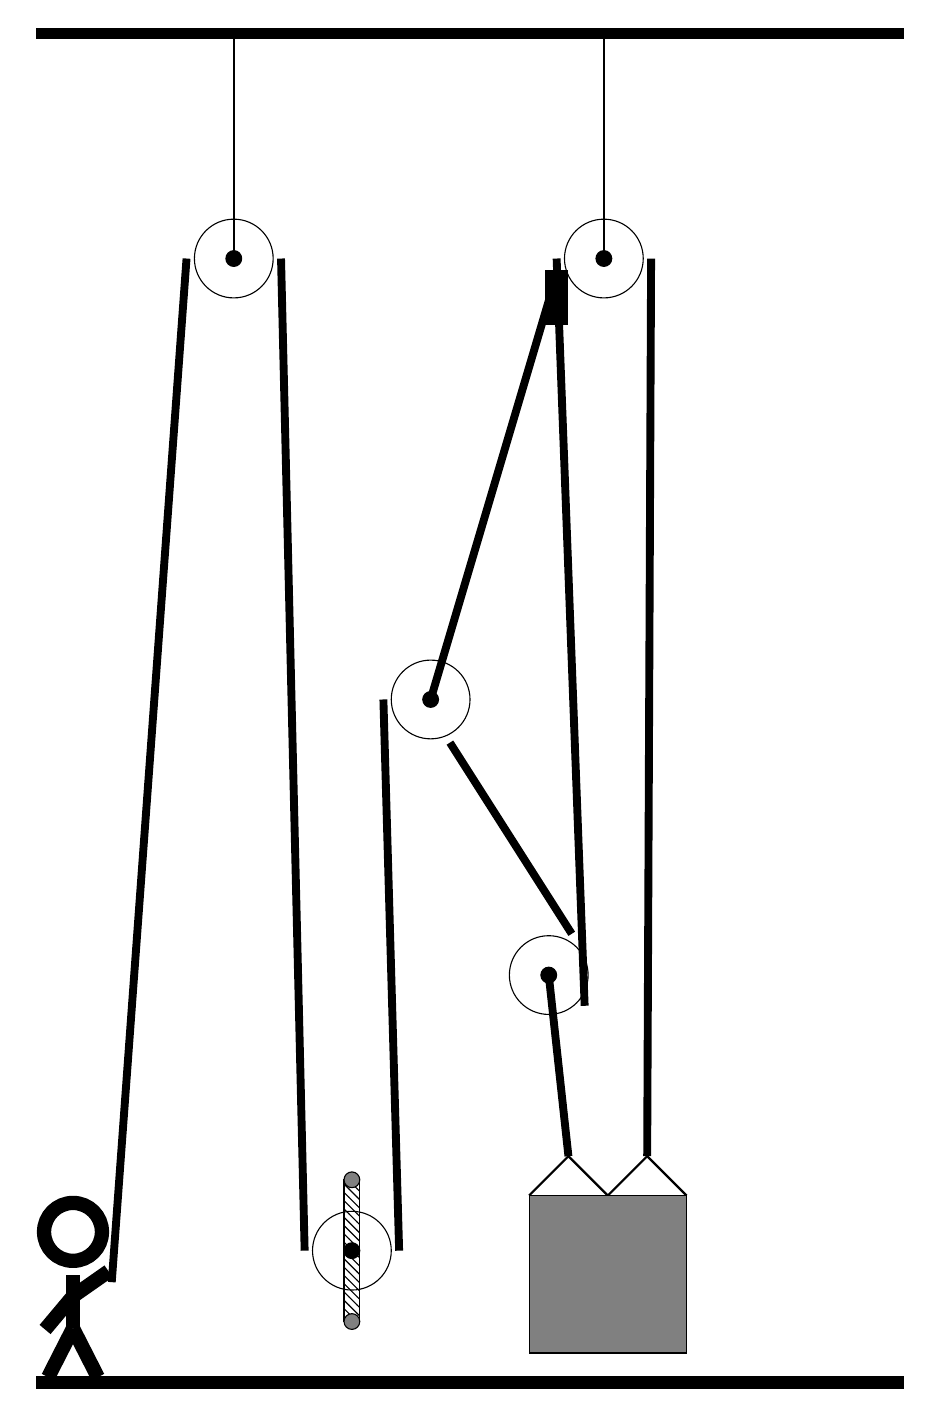
\begin{tikzpicture}
		%%%%% START %%%%%
		\draw[fill=black] (-6, 14) rectangle (5, 14.125);
		
		\draw (-1, 5.6) circle (0.5);
		\draw[fill=black] (-1, 5.6) circle (0.1);
		
		\draw (0.5, 2.1) circle (0.5);
		\draw[fill=black] (0.5, 2.1) circle (0.1);
		
		\draw (1.2, 11.2) circle (0.5);
		\draw[fill=black] (1.2, 11.2) circle (0.1);
		\draw[thick] (1.2, 11.2) -- (1.2, 14);
		
		\draw (-3.5, 11.2) circle (0.5);
		\draw[fill=black] (-3.5, 11.2) circle (0.1);
		\draw[thick] (-3.5, 11.2) -- (-3.5, 14);
		
		\draw (-2, -1.4) circle (0.5);
		\draw[fill=black] (-2, -1.4) circle (0.1);
		\draw[pattern=north west lines, pattern color=black] (-2.1, -0.5) rectangle (-1.9, -2.3);
		\draw[fill=black!50] (-2, -0.5) circle (0.1);
		\draw[fill=black!50] (-2, -2.3) circle (0.1);
		
		\draw[thick]  (0.25, -0.7) -- (0.75, -0.2) -- (1.25, -0.7) -- (1.75, -0.2) -- (2.25, -0.7);
		\draw[fill=black!50] (0.25, -0.7) rectangle (2.25, -2.7);
		\draw[line width=1mm] (-5.05, -1.8) -- (-4.1, 11.2);
		\centerarc[line width=1mm](-3.5, 11.2)(0:180:0.6);
		\draw[line width=1mm] (-2.9, 11.2) -- (-2.6, -1.4);
		\centerarc[line width=1mm](-2, -1.4)(180:360:0.6);
		\draw[line width=1mm] (-1.4, -1.4) -- (-1.6, 5.6);
		\draw[line width=1mm] (-1, 5.6) -- (0.6, 11.0);
		\draw[line width=1mm, fill=black](0.5, 10.4) rectangle (0.7, 11.0);
		\centerarc[line width=1mm](-1, 5.6)(-20:180:0.6);
		\draw[line width=1mm] (-0.755, 5.052) -- (0.792, 2.624);
		\centerarc[line width=1mm](0.5, 2.1)(160:380:0.6);
		\draw[line width=1mm] (0.956, 1.71) -- (0.6, 11.2);
		\draw[line width=1mm](0.5, 2.1) -- (0.75, -0.2);
		\centerarc[line width=1mm](1.2, 11.2)(0:180:0.6);
		\draw[line width=1mm] (1.8, 11.2) -- (1.75, -0.2);
		
		\node at (-5.5, -1.9) {\Strichmaxerl[10][50][35]};
		
		\draw[fill=black] (-6, -3) rectangle (5, -3.15);
		%%%%% END %%%%%
	\end{tikzpicture}
\end{document}